\documentclass[Absender, version=last]{scrlttr2}

%----------------------------------------------------------------------------------------
%	Pakete
%----------------------------------------------------------------------------------------

\usepackage[utf8]{inputenc}
\usepackage[ngerman]{babel}
\usepackage[T1]{fontenc}

%----------------------------------------------------------------------------------------
%	Befehle
%----------------------------------------------------------------------------------------

\KOMAoptions{
	paper=a4,
	fontsize=12pt
}

\hypersetup{
	%pdftitle= \textbar{} Jan Hoegen,
	pdfauthor=Jan Hoegen, 
	%pdfsubject=
}

\setkomavar{signature}{
	\\
	\vspace{-3em}
	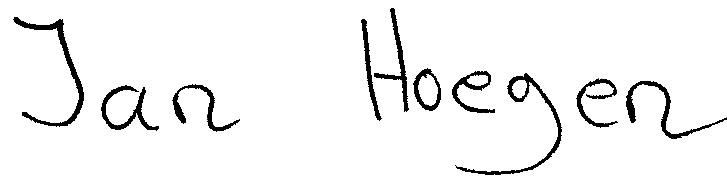
\includegraphics[width=0.35\textwidth]{Signatur.png}}

%----------------------------------------------------------------------------------------
%	Oberes Drittel
%----------------------------------------------------------------------------------------

\begin{document}

\begin{letter}{%
	Stadt Walldorf\\
	Postfach 105520\\
	69045 Heidelberg
}

\setkomavar{place}{Walldorf}

\setkomavar{date}{\today}

\setkomavar{myref}{505}

%\setkomavar{title}{Corona-Verordnung Sportstätten}

\setkomavar{subject}{Abgabe des Führerscheins}

%\setkomavar{firstfoot}{Dies ist die erste Fußzeile}

%----------------------------------------------------------------------------------------
%	Text
%----------------------------------------------------------------------------------------

\opening{Sehr geehrte Damen und Herren,}

hiermit reiche ich meinen Führerschein bei Ihnen ein. 
hiermit reiche ich Ihnen den \textit{Nachweis über die Teilnahme an einem Studienorientierungsverfahren} nach. Dieser wurde auf der Website \texttt{was-studiere-ich.de} durchgeführt.\par
Meine Bewerbernummer lautet: \textbf{6.604.434}

%----------------------------------------------------------------------------------------
%	Unteres Drittel
%----------------------------------------------------------------------------------------

\closing{Mit freundlichen Grüßen,}

%\ps PS: Noch einen schönen Abend.

\encl{Teilnahmezertifikat \texttt{was-studiere-ich.de}}

%\cc{Ich}


%----------------------------------------------------------------------------------------
%	Ende
%----------------------------------------------------------------------------------------

\end{letter}
\end{document}